\documentclass[border=10pt]{standalone}
\usepackage{tikz}
\usepackage{amsmath}
\usetikzlibrary{arrows.meta}

\begin{document}
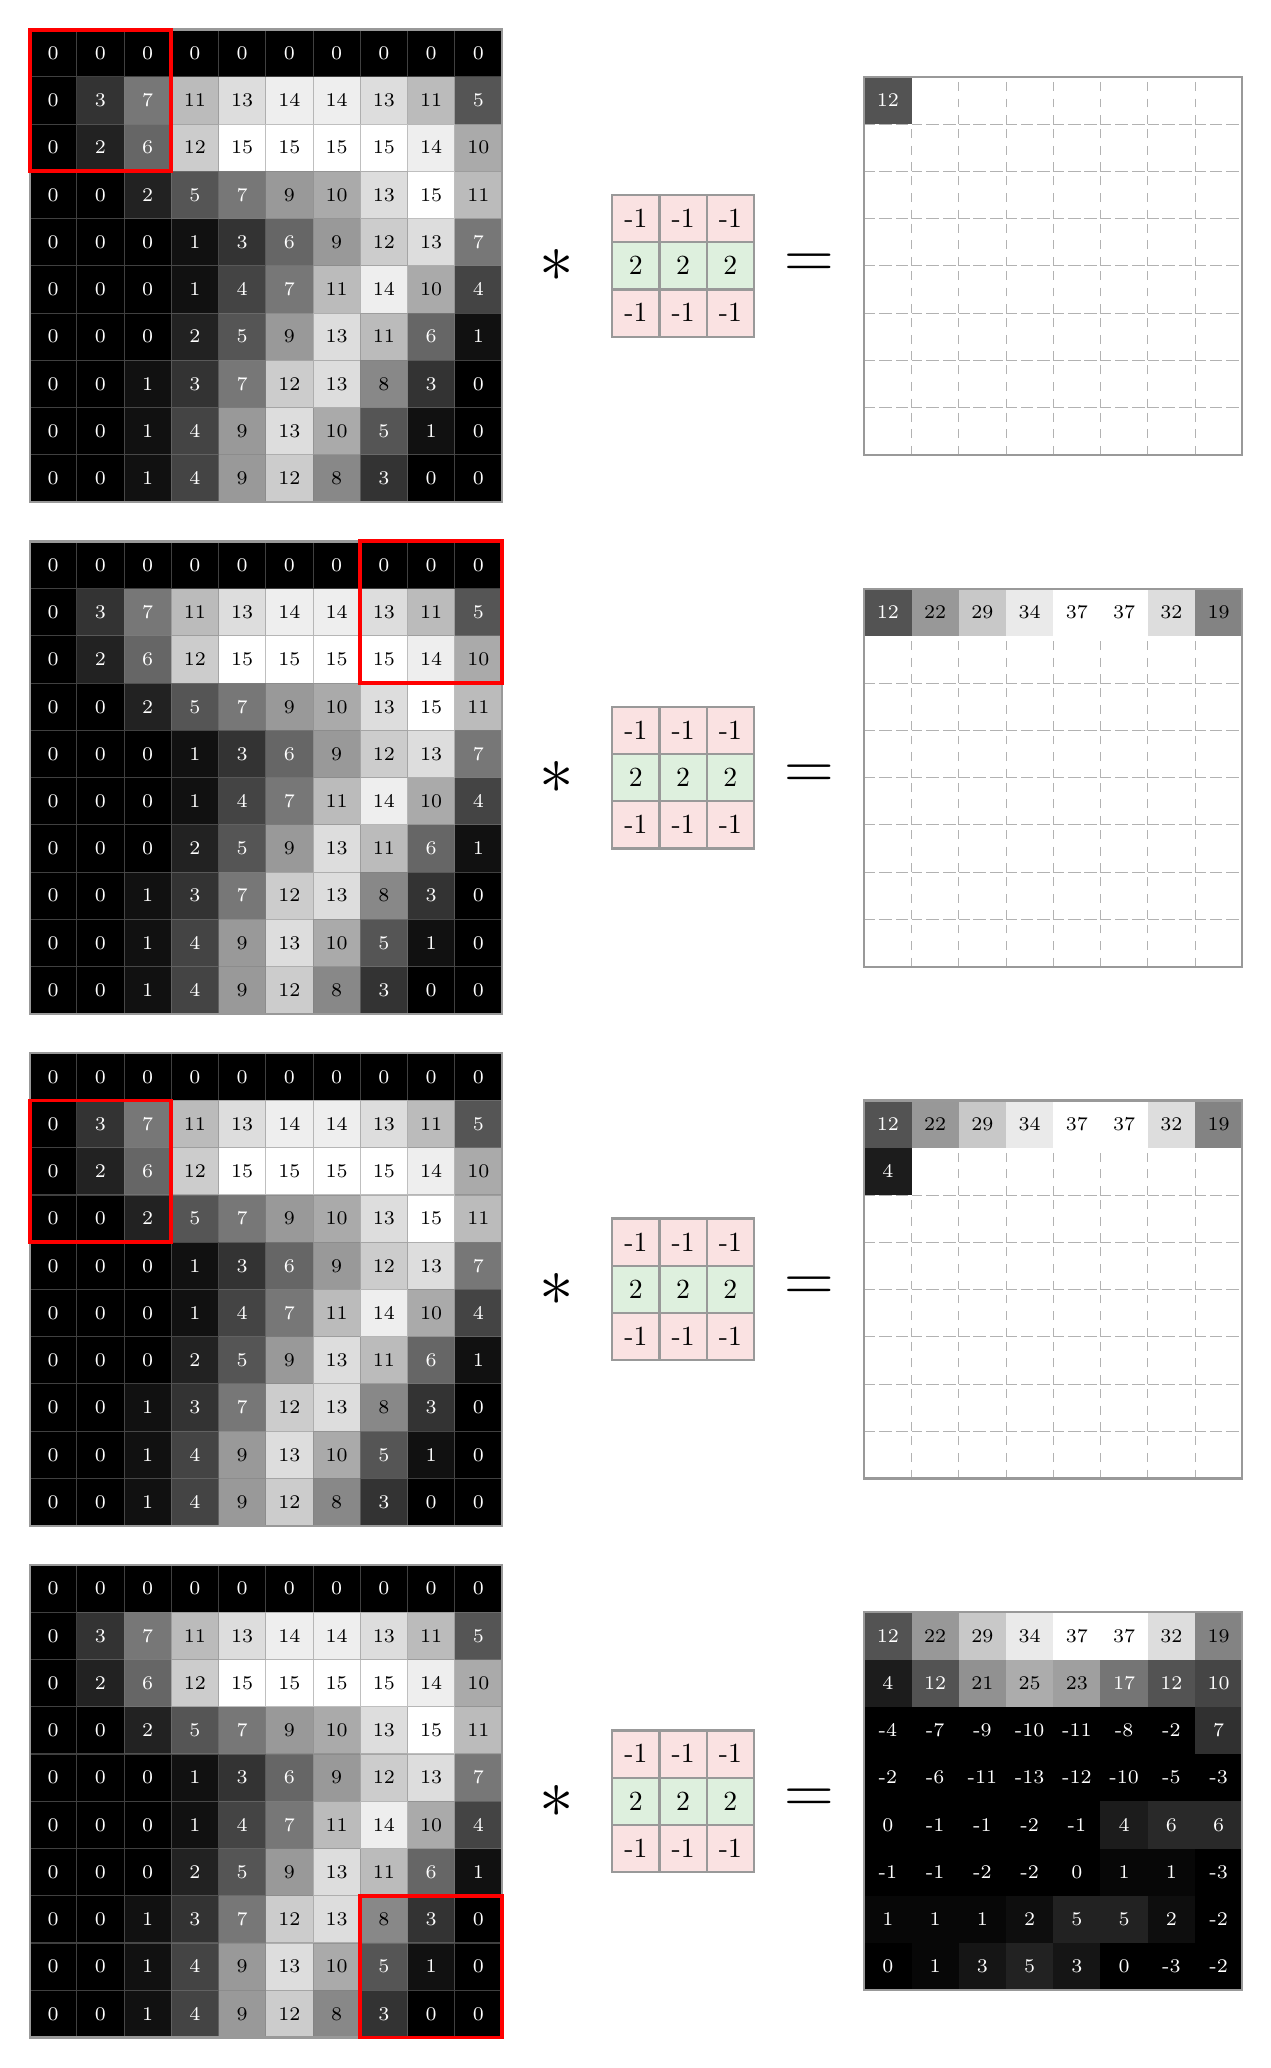
\begin{tikzpicture}[>={Stealth[length=4pt]}, line width=0.8pt, font=\large]

  % ========== 可复用：带数字的 10x10 图（格 0.6，#1 = y 偏移） ==========
  \newcommand{\drawimage}[1]{%
    \foreach \v [count=\n] in {%
      0,0,0,0,0,0,0,0,0,0,%
      0,3,7,11,13,14,14,13,11,5,%
      0,2,6,12,15,15,15,15,14,10,%
      0,0,2,5,7,9,10,13,15,11,%
      0,0,0,1,3,6,9,12,13,7,%
      0,0,0,1,4,7,11,14,10,4,%
      0,0,0,2,5,9,13,11,6,1,%
      0,0,1,3,7,12,13,8,3,0,%
      0,0,1,4,9,13,10,5,1,0,%
      0,0,1,4,9,12,8,3,0,0%
    }{%
      \pgfmathtruncatemacro{\col}{int(mod(\n-1,10))}
      \pgfmathtruncatemacro{\row}{int((\n-1)/10)}
      \pgfmathsetmacro{\gpct}{\v/15}
      \definecolor{px}{gray}{\gpct}
      \fill[px] ({0.6*\col}, {#1+0.6*(9-\row)}) rectangle ++(0.6,0.6);
      \ifnum\v>7 \def\tc{black}\else \def\tc{white}\fi
      \node[font=\scriptsize, text=\tc] at ({0.6*\col+0.3}, {#1+0.6*(9-\row)+0.3}) {\v};
    }
    \begin{scope}[shift={(0,#1)}]
      \draw[gray, opacity=0.5, thin, step=0.6] (0,0) grid (6,6);
      \draw[gray!80] (0,0) rectangle (6,6);
    \end{scope}
  }

  % ========== 可复用：红框（#1=y偏移, #2=顶行, #3=左列） ==========
  \newcommand{\drawbox}[3]{%
    \draw[red, line width=1.4pt] ({0.6*(#3-1)}, {#1+0.6*(8-#2)}) rectangle ({0.6*(#3+2)}, {#1+0.6*(11-#2)});
  }

  % ========== 可复用：3x3 卷积核 ==========
  \newcommand{\drawkernel}[2]{%
    \foreach \w [count=\m] in {-1,-1,-1,2,2,2,-1,-1,-1} {%
      \pgfmathtruncatemacro{\kc}{int(mod(\m-1,3))}
      \pgfmathtruncatemacro{\kr}{int((\m-1)/3)}
      \ifnum\w>0 \definecolor{kw}{RGB}{222,240,222}\else \definecolor{kw}{RGB}{250,226,226}\fi
      \fill[kw] ({#1+0.6*\kc}, {#2+0.6*(2-\kr)}) rectangle ++(0.6,0.6);
      \node[font=\normalsize] at ({#1+0.6*\kc+0.3}, {#2+0.6*(2-\kr)+0.3}) {\w};
    }
    \begin{scope}[shift={(#1,#2)}]
      \draw[gray!80, step=0.6] (0,0) grid (1.8,1.8);
      \draw[gray!80] (0,0) rectangle (1.8,1.8);
    \end{scope}
  }

  % ========== 可复用：8x8 结果灰度图（部分填充；#3 = 一层花括号的 行/列/值 列表） ==========
  \newcommand{\drawresult}[3]{%
    \foreach \r in {0,...,7} \foreach \c in {0,...,7}
      \draw[gray!60, dashed, line width=0.3pt] ({#1+0.6*\c}, {#2+0.6*\r}) rectangle ++(0.6,0.6);
    \foreach \a/\b/\v in {#3} {%
      \pgfmathsetmacro{\g}{max(0, min(\v/37, 1))}
      \definecolor{oc}{gray}{\g}
      \ifdim\g pt>0.5pt \def\tc{black}\else \def\tc{white}\fi
      \fill[oc] ({#1+0.6*(\b-1)}, {#2+0.6*(8-\a)}) rectangle ++(0.6,0.6);
      \node[font=\scriptsize, text=\tc] at ({#1+0.6*(\b-1)+0.3}, {#2+0.6*(8-\a)+0.3}) {\v};
    }%
    \draw[gray!80] (#1,#2) rectangle ({#1+4.8}, {#2+4.8});
  }

  % ========== 可复用：8x8 结果灰度图（全填充；#3 = 一层花括号的 64 个值） ==========
  \newcommand{\drawresultfull}[3]{%
    \foreach \v [count=\n] in {#3} {%
      \pgfmathtruncatemacro{\r}{int((\n-1)/8)}
      \pgfmathtruncatemacro{\c}{int(mod(\n-1,8))}
      \pgfmathsetmacro{\g}{max(0, min(\v/37, 1))}
      \definecolor{oc}{gray}{\g}
      \ifdim\g pt>0.5pt \def\tc{black}\else \def\tc{white}\fi
      \fill[oc] ({#1+0.6*\c}, {#2+0.6*(7-\r)}) rectangle ++(0.6,0.6);
      \node[font=\scriptsize, text=\tc] at ({#1+0.6*\c+0.3}, {#2+0.6*(7-\r)+0.3}) {\v};
    }%
    \draw[gray!80] (#1,#2) rectangle ({#1+4.8}, {#2+4.8});
  }

  % ================= 第一行（★ 偏移 21->19.5，中心 24->22.5） =================
  \drawimage{19.5}  \drawbox{19.5}{1}{1}
  \node[font=\Huge] at (6.7,22.5) {$\ast$};
  \drawkernel{7.4}{21.6}
  \node[font=\Huge] at (9.9,22.5) {$=$};
  \drawresult{10.6}{20.1}{1/1/12}

  % ================= 第二行（★ 偏移 14->13，中心 17->16） =================
  \drawimage{13}  \drawbox{13}{1}{8}
  \node[font=\Huge] at (6.7,16) {$\ast$};
  \drawkernel{7.4}{15.1}
  \node[font=\Huge] at (9.9,16) {$=$};
  \drawresult{10.6}{13.6}{1/1/12,1/2/22,1/3/29,1/4/34,1/5/37,1/6/37,1/7/32,1/8/19}

  % ================= 第三行（★ 偏移 7->6.5，中心 10->9.5） =================
  \drawimage{6.5}  \drawbox{6.5}{2}{1}
  \node[font=\Huge] at (6.7,9.5) {$\ast$};
  \drawkernel{7.4}{8.6}
  \node[font=\Huge] at (9.9,9.5) {$=$};
  \drawresult{10.6}{7.1}{1/1/12,1/2/22,1/3/29,1/4/34,1/5/37,1/6/37,1/7/32,1/8/19,2/1/4}

  % ================= 第四行（不变，中心 y=3） =================
  \drawimage{0}  \drawbox{0}{8}{8}
  \node[font=\Huge] at (6.7,3) {$\ast$};
  \drawkernel{7.4}{2.1}
  \node[font=\Huge] at (9.9,3) {$=$};
  \drawresultfull{10.6}{0.6}{%
    12,22,29,34,37,37,32,19,%
    4,12,21,25,23,17,12,10,%
    -4,-7,-9,-10,-11,-8,-2,7,%
    -2,-6,-11,-13,-12,-10,-5,-3,%
    0,-1,-1,-2,-1,4,6,6,%
    -1,-1,-2,-2,0,1,1,-3,%
    1,1,1,2,5,5,2,-2,%
    0,1,3,5,3,0,-3,-2}
\end{tikzpicture}
\end{document}